\chapter{Proposed Sintactic and Semantic Analyzer}
\label{ch:proposed-sin-sema-anal}
After analyzing the existing tools, we can see that different
aspects of existing technology can be improved, such as those
discussed in \cref{sec:anal-enhacements}. In this section we will make a proposal
for a system solution, evaluating each of the aspects to be
improved and we will model, through use cases and requirements,
what aspects a system that would like to respond to the analyzed
problem should meet.

\section{Enhancement of error messages}
After analyzing the existing tools, one of the aspects that we have
observed that can be improved is the content of the error messages.
\cite{heeren2005top} refers to the most relevant points that an error message must
have to convey the entire context. First, it must contain the
location in the form of a file, line and position on the line.
In addition, it is highly recommended, according to \cite{heeren2005top}, that the
error context be added, this is the piece of code that generated
the error. They qualify as essential to give a generic error
message and if others can be enriched with more information 
uch as within the code fragment that generated the error,
which part caused it and why, the better.

From everything previously done and from this last small summary we can say
that a system that wants to improve all these aspects will have to comply
with the following use cases (\cref{fig:enh-err-use-case}).

\begin{figure}[h!]
    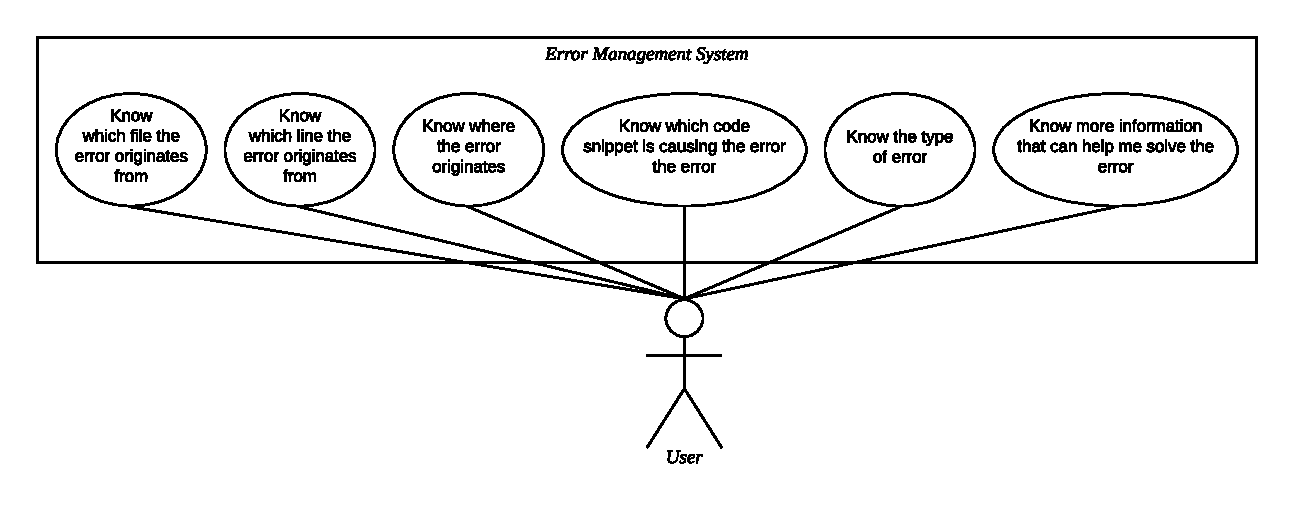
\includegraphics[scale=0.6]{images/enh-err-use-case.pdf}
    \centering
    \caption[Use cases extracted from improving error messages]{Use cases extracted from improving error messages.}
    \label{fig:enh-err-use-case}
\end{figure}

In addition, these use cases emanate or we can extract high-level
requirements that will help us guide the implementation of the system.

\begin{figure}[h!]
    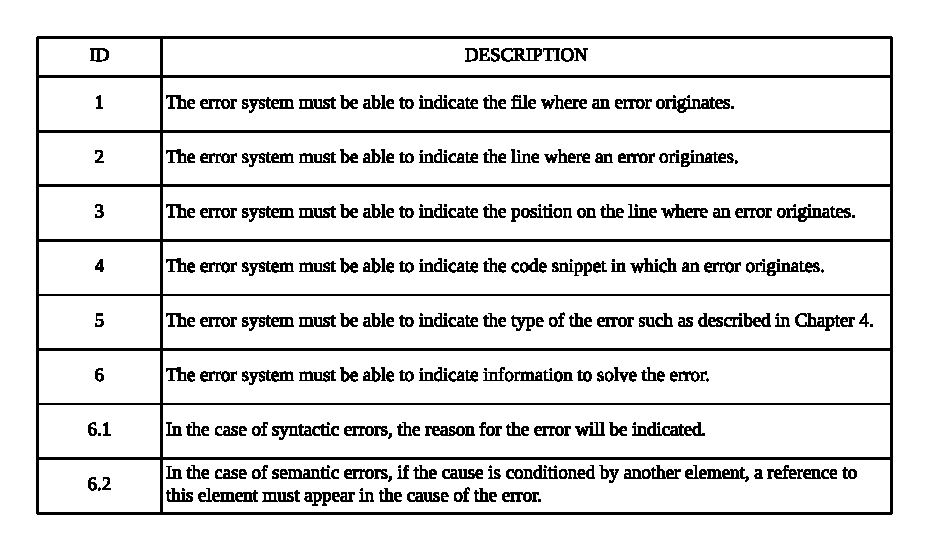
\includegraphics[width=\textwidth]{images/enh-err-requirements.pdf}
    \centering
    \caption[Requirements extracted from improving error messages]{Requirements extracted from improving error messages.}
    \label{fig:enh-err-req}
\end{figure}

\section{Creation of the warning type message}
Another aspect that can be improved in syntactic and semantic analysis
is adding a new type of error message that, while not as serious as an
error, represents an upgradeable aspect of the system. For this purpose,
the creation of a new type of error message (which implies that it
should comply with the requirements of the previous point) of the
warning type is proposed. The following use case models the system that
should contain this type of error

\begin{figure}[h!]
    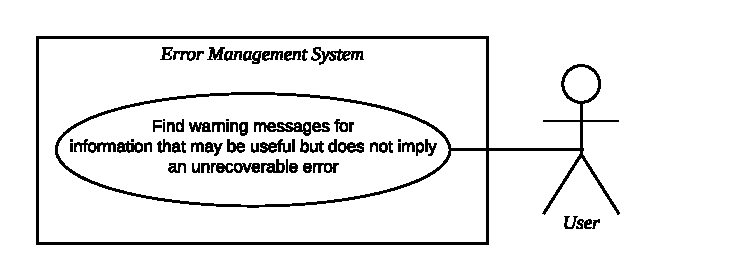
\includegraphics[scale=0.8]{images/warn-use-case.pdf}
    \centering
    \caption[Use cases extracted from new warning message type]{Use cases extracted from new warning message type.}
    \label{fig:warn-use-case}
\end{figure}

And therefore we can extract the following requirement for a future system.

\begin{figure}[h!]
    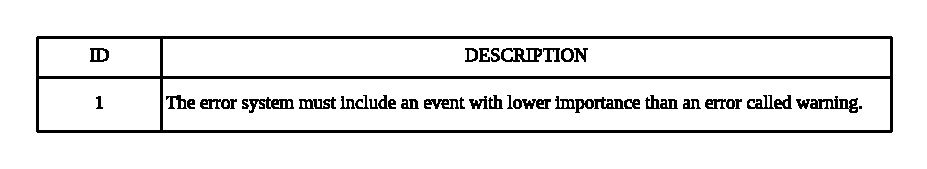
\includegraphics[scale=0.8]{images/warn-req.pdf}
    \centering
    \caption[Requirements extracted from new warning message type]{Requirements extracted from new warning message type.}
    \label{fig:warn-req}
\end{figure}

\section{Detection of override definitions}
As stated in the analysis, it is interesting to be able to include detection of
definitions that overwrite each other. For this, the use case in which a future
system will support is defined below.

\begin{figure}[h!]
    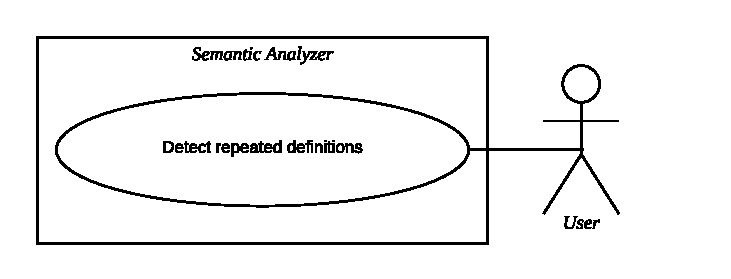
\includegraphics[scale=0.8]{images/def-override-use-case.pdf}
    \centering
    \caption[Use cases extracted from detection of override definitions]{Use cases extracted from detection of override definitions.}
    \label{fig:def-overr-use-case}
\end{figure}

And therefore we can extract the following requirement for a future system.

\begin{figure}[h!]
    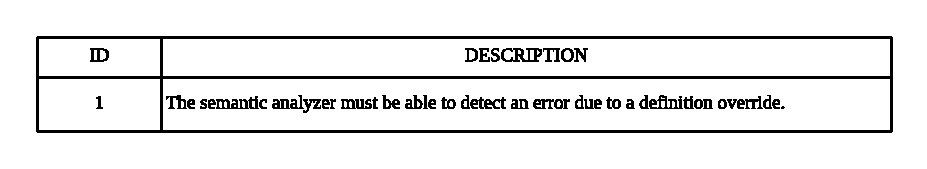
\includegraphics[scale=0.8]{images/def-override-req.pdf}
    \centering
    \caption[Requirements extracted from detection of override definitions]{Requirements extracted from detection of override definitions.}
    \label{fig:def-overr-req}
\end{figure}

\section{Detection of undefined references}
As mentioned in the analysis, the detection of undefined references is
important to validate a scheme, therefore the use cases and requirements
to implement a future system are modeled below.

\begin{figure}[h!]
    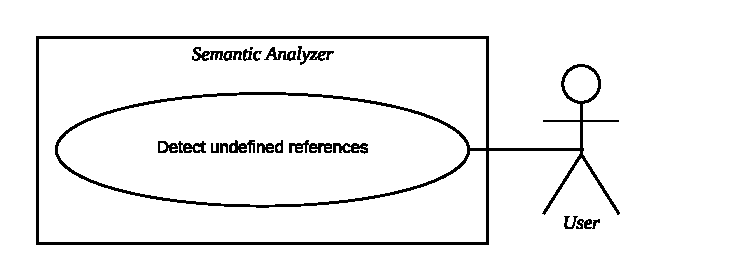
\includegraphics[scale=0.8]{images/und-ref-use-case.pdf}
    \centering
    \caption[Use cases extracted from detection of undefined references]{Use cases extracted from detection of undefined references.}
    \label{fig:und-ref-use-case}
\end{figure}

And therefore we can extract the following requirement for a future system.

\begin{figure}[h!]
    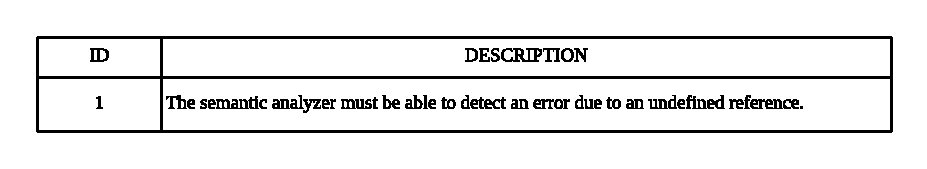
\includegraphics[scale=0.8]{images/und-ref-req.pdf}
    \centering
    \caption[Requirements extracted from detection of undefined references]{Requirements extracted from detection of undefined references.}
    \label{fig:und-ref-req}
\end{figure}

\section{Detection of unused resources}
In order to detect non-used resources, it is not necessary that
the error message be of type error, it should be of type warning.
The following use case and requirement model this situation.

\begin{figure}[h!]
    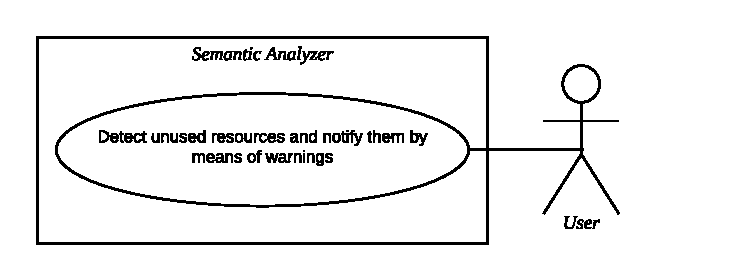
\includegraphics[scale=0.8]{images/unu-res-use-case.pdf}
    \centering
    \caption[Use cases extracted from detection of unused resources]{Use cases extracted from detection of unused resources.}
    \label{fig:unu-res-use-case}
\end{figure}

And therefore we can extract the following requirement for a future system.

\begin{figure}[h!]
    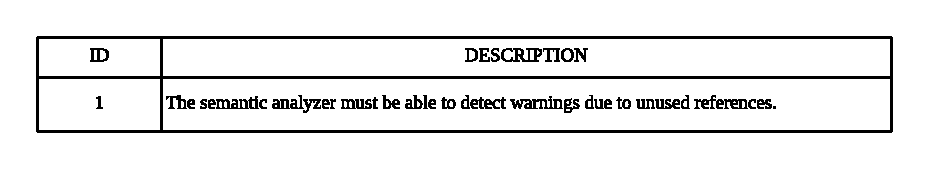
\includegraphics[scale=0.8]{images/unu-res-req.pdf}
    \centering
    \caption[Requirements extracted from detection of unused resources]{Requirements extracted from detection of unused resources.}
    \label{fig:unu-res-req}
\end{figure}

\section{Detection of multiple errors / warnings at once}
In order to meet the objective of detecting multiple errors at the same
time, any system must meet the following use case and the requirements
that arise from it.

\begin{figure}[h!]
    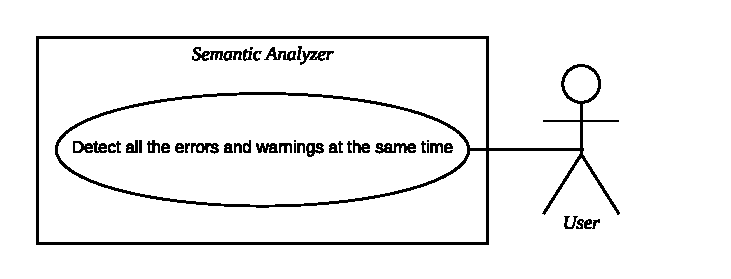
\includegraphics[scale=0.8]{images/mul-err-use-case.pdf}
    \centering
    \caption[Use cases extracted from detection of multiple errors / warnings at once]{Use cases extracted from detection of multiple errors / warnings at once.}
    \label{fig:mul-err-use-case}
\end{figure}

And therefore we can extract the following requirement for a future system.

\begin{figure}[h!]
    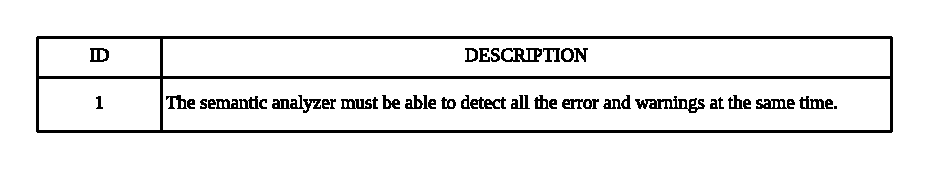
\includegraphics[scale=0.8]{images/mul-err-req.pdf}
    \centering
    \caption[Requirements extracted from detection of multiple errors / warnings at once]{Requirements extracted from detection of multiple errors / warnings at once.}
    \label{fig:mul-err-req}
\end{figure}